%% abtex2-modelo-artigo.tex, v-1.9.2 laurocesar
%% Copyright 2012-2014 by abnTeX2 group at http://abntex2.googlecode.com/ 
%%
%% This work may be distributed and/or modified under the
%% conditions of the LaTeX Project Public License, either version 1.3
%% of this license or (at your option) any later version.
%% The latest version of this license is in
%%   http://www.latex-project.org/lppl.txt
%% and version 1.3 or later is part of all distributions of LaTeX
%% version 2005/12/01 or later.
%%
%% This work has the LPPL maintenance status `maintained'.
%% 
%% The Current Maintainer of this work is the abnTeX2 team, led
%% by Lauro César Araujo. Further information are available on 
%% http://abntex2.googlecode.com/
%%
%% This work consists of the files abntex2-modelo-artigo.tex and
%% abntex2-modelo-references.bib
%%

% ------------------------------------------------------------------------
% ------------------------------------------------------------------------
% abnTeX2: Modelo de Artigo Acadêmico em conformidade com
% ABNT NBR 6022:2003: Informação e documentação - Artigo em publicação 
% periódica científica impressa - Apresentação
% ------------------------------------------------------------------------
% ------------------------------------------------------------------------

\documentclass[
	% -- opções da classe memoir --
	article,			% indica que é um artigo acadêmico
	11pt,				% tamanho da fonte
	oneside,			% para impressão apenas no verso. Oposto a twoside
	a4paper,			% tamanho do papel. 
	% -- opções da classe abntex2 --
	%chapter=TITLE,		% títulos de capítulos convertidos em letras maiúsculas
	%section=TITLE,		% títulos de seções convertidos em letras maiúsculas
	%subsection=TITLE,	% títulos de subseções convertidos em letras maiúsculas
	%subsubsection=TITLE % títulos de subsubseções convertidos em letras maiúsculas
	% -- opções do pacote babel --
	english,			% idioma adicional para hifenização
	brazil,				% o último idioma é o principal do documento
	sumario=tradicional
	]{abntex2}


% ---
% PACOTES
% ---

% ---
% Pacotes fundamentais 
% ---
\usepackage{lmodern}			% Usa a fonte Latin Modern
\usepackage[T1]{fontenc}		% Selecao de codigos de fonte.
\usepackage[utf8]{inputenc}		% Codificacao do documento (conversão automática dos acentos)
\usepackage{indentfirst}		% Indenta o primeiro parágrafo de cada seção.
\usepackage{nomencl} 			% Lista de simbolos
\usepackage{color}				% Controle das cores
\usepackage{graphicx}			% Inclusão de gráficos
\usepackage{microtype} 			% para melhorias de justificação
% ---
		
% ---
% Pacotes adicionais, usados apenas no âmbito do Modelo Canônico do abnteX2
% ---
\usepackage{lipsum}				% para geração de dummy text
% ---
		
% ---
% Pacotes de citações
% ---
\usepackage[brazilian,hyperpageref]{backref}	 % Paginas com as citações na bibl
\usepackage[alf]{abntex2cite}	% Citações padrão ABNT
% ---

% ---
% Configurações do pacote backref
% Usado sem a opção hyperpageref de backref
\renewcommand{\backrefpagesname}{Citado na(s) página(s):~}
% Texto padrão antes do número das páginas
\renewcommand{\backref}{}
% Define os textos da citação
\renewcommand*{\backrefalt}[4]{
	\ifcase #1 %
		Nenhuma citação no texto.%
	\or
		Citado na página #2.%
	\else
		Citado #1 vezes nas páginas #2.%
	\fi}%
% ---

% ---
% Informações de dados para CAPA e FOLHA DE ROSTO
% ---
\titulo{Uma proposta de método para análise e desenho de uma Arquitetura Orientada a Serviços}
\autor{José Valdvogel de Almeida Junior
\thanks{valdvogel@hotmail.com}}
\local{Brasil}
\data{2014, v-1.0}
% ---

% ---
% Configurações de aparência do PDF final

% alterando o aspecto da cor azul
\definecolor{blue}{RGB}{41,5,195}

% informações do PDF
\makeatletter
\hypersetup{
     	%pagebackref=true,
		pdftitle={\@title}, 
		pdfauthor={\@author},
    	pdfsubject={Arquitetura Orientada a Serviços},
	    pdfcreator={LaTeX with abnTeX2},
		pdfkeywords={abnt}{latex}{abntex}{abntex2}{atigo científico}, 
		colorlinks=true,       		% false: boxed links; true: colored links
    	linkcolor=blue,          	% color of internal links
    	citecolor=blue,        		% color of links to bibliography
    	filecolor=magenta,      		% color of file links
		urlcolor=blue,
		bookmarksdepth=4
}
\makeatother
% --- 

% ---
% compila o indice
% ---
\makeindex
% ---

% ---
% Altera as margens padrões
% ---
\setlrmarginsandblock{3cm}{3cm}{*}
\setulmarginsandblock{3cm}{3cm}{*}
\checkandfixthelayout
% ---

% --- 
% Espaçamentos entre linhas e parágrafos 
% --- 

% O tamanho do parágrafo é dado por:
\setlength{\parindent}{1.3cm}

% Controle do espaçamento entre um parágrafo e outro:
\setlength{\parskip}{0.2cm}  % tente também \onelineskip

% Espaçamento simples
\SingleSpacing

% ----
% Início do documento
% ----
\begin{document}

% Retira espaço extra obsoleto entre as frases.
\frenchspacing 

% ----------------------------------------------------------
% ELEMENTOS PRÉ-TEXTUAIS
% ----------------------------------------------------------

%---
%
% Se desejar escrever o artigo em duas colunas, descomente a linha abaixo
% e a linha com o texto ``FIM DE ARTIGO EM DUAS COLUNAS''.
\twocolumn[    		% INICIO DE ARTIGO EM DUAS COLUNAS
%
%---
% página de titulo
\maketitle

% resumo em português
\begin{resumoumacoluna}
Com a evolução tecnologica e o aumento  da computação distribuida a arquitetura orientada a serviço (SOA) tem se tornado uma abordagem cada vez mais utilizada como paradgima arquitetural para projetos de software. No entanto, alguns projetos que utilizam esse paradigma não obtiveram sucesso na sua adoção pelo fato de sua aplicação ir além dos limites tecnologicos. Esse trabalho visa estudar os problemas ocorridos e realizar uma proposta de método que auxilie arquitetos de software a montar um processo de desenvolvimento voltados para os princípios do paradigma orientado a serviço.
 
 \vspace{\onelineskip}
 
 \noindent
 \textbf{Palavras-chaves}: SOA. Modelagem. Serviço. Catalysis. Arquitetura.
\end{resumoumacoluna}

 ]  				% FIM DE ARTIGO EM DUAS COLUNAS
% ---

% ----------------------------------------------------------
% ELEMENTOS TEXTUAIS
% ----------------------------------------------------------
\textual

% ----------------------------------------------------------
% Introdução
% ----------------------------------------------------------
\section*{Introdução}
\addcontentsline{toc}{section}{Introdução}

Problemas na construção de software são desafios recorrentes desde que o desenvolvimento de aplicações tornou os processos de negócio mais ágeis e o investimento em TI uma necessidade. Estudos econômicos na década de noventa concluiram que a produção e o uso de TI contribuiu em mais da métade para o crescimento da produtividades americana e que o investimento em software subiu de US\$ 82 bilhões de dólares em 1995 para US\$149 bilhões em 1999 \cite{CynthiaKRiemenschneider2002}.Os gastos com tecnologia da informação no Brasil atingirão US\$ 125,3 bilhões em 2015. A estimativa, divulgada pelo Gartner, aponta para um crescimento da ordem de 5,7\% sobre os US\$ 118,5 bilhões projetados pela consultoria para 2014. Os gastos mundiais vão superar US\$ 3,9 trilhões em 2015, um aumento de 3,9\% em relação a 2014. \cite{ComputerWorld2014}. 
Com base nessa demanda o desenvolvimento de software ganhou um papel de importante destaque na vida organizacional de qualquer empresa.

Arquitetura orientada a serviço (SOA) atualmente é muito utilizada em empresas de diversos ramos que pretendem criar estruturas de software com flexibidade, integridade e reuso. No entanto, muito dessas empresas fracassam devido a trabalharem da mesma forma que trabalhavam com outros estilos arquiteturais. As estruturas e processos de sistemas antigos são inadequados e podem portanto levar a uma desaceleração ou perda de oportunidades\cite{Rothenberger2010}. Esse artigo tenta propor um método para construção de software quando SOA é sugerido como estilo arquitetural para empresas que precisam de funcionalidade altamente distribuida, arquitetura desacoplada e padronização de interfaces.


% ----------------------------------------------------------
% Pequena Introdução sobre SOA
% ----------------------------------------------------------
\newpage
\section{Arquitetura Orientada a Serviço}

Existem várias definições para SOA e normalmente ela esta associada à tecnologia Web Services, porém sua definição vai muito além, pois está em torno de conjunto de princípios e padrões. SOA é uma arquitetura de software que define o uso de serviços para dar suporte aos requisitos do usuário\cite{Lee2006}. As características desses serviços são baixo acoplamento, contrato de serviço, autonômia, abstração, reuso, composição, gerenciamento de estado e descoberta\cite{Erl2005}. Características essas oriundas da orientação de objetos e da computação distríbuida que visam aspectos de hardware com máquina independentes e autônamas, e software onde um determinado sistema se apresenta ao usuário como uma única máquina. Características que se fazem presente atualmente pelo crescimento tecnologico, mas que por outro lado vem apresentando problemas constantes pelo fato de os métodos utilizados para sua concepção serem os mesmos.

% ----------------------------------------------------------
% Método (Como ?)
% ----------------------------------------------------------
\section{Desafios nas fases de desenvolvimento}
Desde a crise de software uma série de métodos foram criados para auxiliar na construção de peças de software voltados para o paradigma de programação procedimental. Com a mudança do paradigma procedimental para o orientado a objeto o foco no desenvolvimento ágil ganhou destaque pela necessidade das empresas serem cada vez mais ágeis. Com isso as metodologias clássicas que continham fases de desenvolvimento bem definitas começaram a ter cortes para atender a demanda no tempo e custo combinados. Cortes que nem sempre trouxeram benefícios para os desenvolvedores  e que por muitas vezes trouxeram problemas para desenvolvedores e clientes. 

De acordo com o estudo realizado por Rothenberger com empresas que haviam adotado SOA como pararadigma arquitetural, algumas mudanças na forma de planejar, analisar, desenhar, implementar e testar serviços foram necessárias para que a iniciativa arquitetural fosse desenvolvida com sucesso, pois foi constatado que existiam diferenças significantes no contexto de SOA com Web services em comparação ao desenvolvimento de software anterior \cite{Rothenberger2010}. Abaixo segue um resumo das fases e as mudanças necessárias para adoção de SOA.

\begin{table}
\centering
\caption{Resumo dos problemas nas fases de desenvolvimento com SOA}
  \begin{tabularx}{\linewidth}{ | l | X |  }
    \hline Fase & Importantes características e mudanças \\ \hline

	Planejamento
	&
   	Experiência empírica; comunicação entre stakeholder e TI; utilização de padrões;
	 \\ \hline
	Análise
	&
  	Necessário mais rigor do que demais arquiteturas;
	 \\ \hline
	Desenho
	&
	Desenho de contratos; Granularidade; Atenção aos serviços remotos;
	 \\ \hline
	Implementação
	&
	Interoperabilidade; Gerenciamento e rastreabilidade;
	 \\ \hline
	Teste
	&
	Ciclo de vida; Segurança ; Desempenho;
	 \\ \hline

  \end{tabularx}
\end{table}

Em seu estudo Rothenberger deixa claro que as fases de planejamento, analise e desenho necessitam de uma abordagem mais tradicional, pois alguns aspectos do desenvolvimento orientado a serviço podem necessitar de mais disciplina e mentalidade holística do que os cenários de desenvolvimento antigos. Dessa perspectiva as abordagens de desenvolvimento ágeis devem constituir uma boa opção para composição de aplicações clientes, enquando os serviços que compõem a infraestrutura podem necessitar de abordagens que enfatizem o planejamento e rigorosos desenhos\cite{Rothenberger2010}. Logo, o foco da pesquisa num primeiro momento é um estudo de um método voltado para construção de componentes em busca de possíveis melhorias para abordagem orientada a serviço. Posteriormente, o estudo de uma abordagem para formalização de processos de negócio e por fim a união entre o processo formal com as fases para o desenvolvimento de componentes.

\subsection{Catalysis}

Catalysis é uma técnica e método que fornece desenvolvimento baseado em componente, desenho de alta integridade, desenho orientado a objeto e reengenharia. Usa notação baseada em padrões indústrias como \textit{Unified Modeling Language} (UML) padronizado pelo \textit{Object Modeling Group} (OMG) \cite{DSouza1998}.
No Catalysis, existem dois conceitos básicos para descrever a análise de desenho dos domínios do usuário. Esses conceitos básicos são os \textit{objetos} que representa um conjunto de informações e funcionalidade e as \textit{ações} representando qualquer coisa que acontece: um evento, trabalho, mensagem, mudança de estado \cite{DSouza1998} conforme indicado na figura 1.

\begin{figure}[h]
	 \centering 
     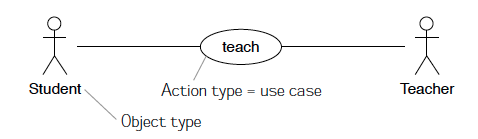
\includegraphics[width=5cm]{Images/fig1.png}
     \caption{Objeto participa de ações}
     \label{Objeto participa de ações}
\end{figure}

Baseado em três constructos básicos - tipo, colaboração e refinamento - fornece a construção de uma grande variedade de modelos e desenhos (ver figura 2). Esses elementos juntos formam um quarto constructo chamado de \textit{framework} que irá representar a união dos constructos em determinado situação.

\begin{figure}[h]
	 \centering 
     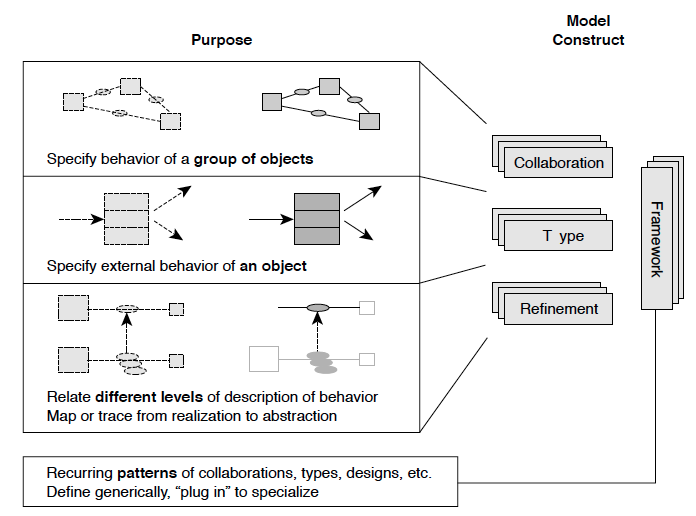
\includegraphics[width=5cm]{Images/fig2.png}
     \caption{Três constructos que padronizam um framework}
     \label{Três constructos que padronizam um framework}
\end{figure}

Tem como base três níveis de modelagem: o domínio do problema ou negócio, o componente ou específicação do sistema (comportamento visível externamente) e o desenho interno do componente ou sistema (estrutura interna e comportamento) indicados na figura 3.

\begin{figure}[h]
	 \centering 
     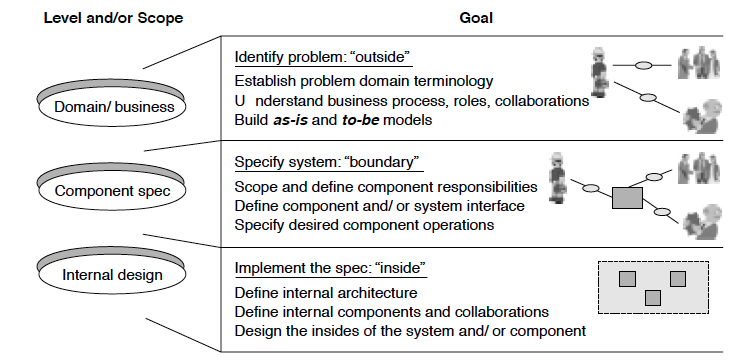
\includegraphics[width=5cm]{Images/fig3.png}
     \caption{Três níveis de modelagem}
     \label{Três níveis de modelagem}
\end{figure}

Assim como SOA é regido por uma série de princípios, o método Catalysis também contém três princípios básicos que fazem parte do seu processo - abstração, precisão e acoplamento. Esses princípios que podem ser vistos na figura 4 e nos guiam como referência para a criação de componentes de software mais integros e flexíveis, pois um software contruido sem o uso de componentes bem definidos será inflexível: dificuldade para mudar quando os requisitos mudam \cite{DSouza1998}.

\begin{figure}[h]
	 \centering 
     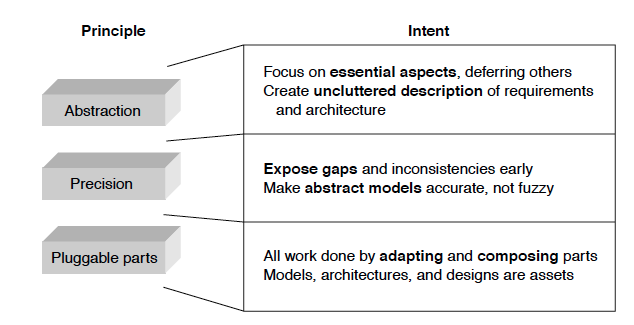
\includegraphics[width=5cm]{Images/fig4.png}
     \caption{Três princípios do Catalysis}
     \label{Três princípios do Catalysis}
\end{figure}

Catalysis contém uma série de características que são comuns a SOA , logo um estudo a partir de seus fundamentos nos auxilia a pensar em meios adaptativos para que as fases de análise e desenho indicadas no estudo como necessidade de mudança sejam realizadas de uma forma segura e bem formada, levando em consideração características básicas como baixo acoplamento e reuso de componentes.

\subsection{BPMN}

Processos de negócio são essênciais para as empresas sobreviverem hoje, pois sem ele falhas de comunição tornam-se constantes. Para evitar esse problema e como uma forma de eliminar as falhas entre negócio e tecnologia evitando os dois maiores problema de falhas em software \cite{International2013}, uma notação que seja de entendimento de negócio e que auxílie na abstração de idéias se faz viável. Para realizar esse papel a notação de processo de negócio \textit{BPMN} se faz relevante para criação de processos formais que auxiliem na comunicação e ampliem o nível de abstração entre negócio e tecnologia. Definimos processos de negócio como uma coleção de atividades que possuem um ou mais insumos e geram um ou mais resultados que representam agregação de valor ao cliente \cite{Hammer2009}. Em geral, um processo de negócio é uma sequência coerente de atividades com o objetivo de executar um serviço. A saída e o resultado de um processo de negócio é um serviço requerido e consumido por um cliente interno ou externo \cite{Scheer1998}.
Com isso, podemos a partir de um processo formal elencar serviços candidatos para infraestrutura da nossa arquitetura assim como serviços que ficarão expostos ao consumo dos clientes.


% ----------------------------------------------------------
% Resultados (O QUE ?	)
% ----------------------------------------------------------
\section{Resultados}

De acordo com os princípios e características apresentadas anteriormente foi proposto ajustes nas fases do método Catalysis com um maior foco nas fases de análise e desenho utilizando notações existente para compor uma nova técnica. Para tal, podemos definir as seguintes fases a seguir apresentadas na figura 5.
\begin{figure}[h]
	 \centering 
     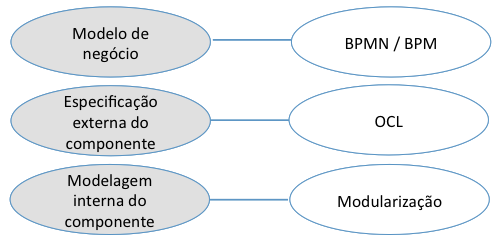
\includegraphics[width=5cm]{Images/fig5.png}
     \caption{Possíveis fases a partir do Catalysis}
     \label{Possíveis fases a partir do Catalysis}
\end{figure}


% ----------------------------------------------------------
% Discussao (Então)
% ----------------------------------------------------------
\section{Discussão}

Como ainda estamos em fase de estudo sobre o método proposto, algumas questões e afirmações em tempo de projeto foram surgindo. Uma dúvida inicial era se o método iria suportar processos informais, porém foi analisado que se não existe uma formalização de processos a abordagem orientada a serviço não é adequada, pois não pode garantir o reuso. Ainda em cima de reuso, existe alguma forma de garantir reuso de um componente nas fases anteriores ao desenvolvimento ?
A partir de um processo formal é possível alguma técnica de descoberta dos possíveis serviços que serão utilizados pela empresa ?
% ---
% Finaliza a parte no bookmark do PDF, para que se inicie o bookmark na raiz
% ---
\bookmarksetup{startatroot}% 
% ---

% ---
% Conclusão
% ---
\section*{Considerações finais}
\addcontentsline{toc}{section}{Considerações finais}
Acredito que o trabalho tem uma grande contribuição para área acadêmica e mercado, pois busca auxílio em um método que foi de grande contribuição para o avanço da modelagem orientada a objeto e que pode ser mais difundida e com grande contribuição para os novos paradigmas e problemas e convivemos hoje.

% ----------------------------------------------------------
% ELEMENTOS PÓS-TEXTUAIS
% ----------------------------------------------------------
\postextual
\newpage
% ----------------------------------------------------------
% Referências bibliográficas
% ----------------------------------------------------------
\bibliography{abntex2-modelo-artigo}

\end{document}
